\section{Implementation}

\begin{frame}
\frametitle{Implementation}
	
	Many interesting implementation details\ldots but we will focus on two:
	\begin{itemize}
		\item Search engine implementation (Lucene).
		\item Application adaptation \& rules description creation (XML/DOM).
	\end{itemize}

\end{frame}

\subsection{Search engine}

\begin{frame}
\frametitle{Search engine}

	First of all, we need to implement the index:
	\begin{itemize}
      	\item From Lucene concepts\ldots 
		\begin{itemize}
      		\item \texttt{Document}
      		\item \texttt{Fields}
        \end{itemize}
        
        \item \ldots to ASTRA concepts: 
		\begin{itemize}
      		\item Astra Application
      		\item some Astra Application attributes (description,type, tags, etc.)
        \end{itemize}
        \item Type of index: \texttt{RAMDirectory}, more efficient and no need
        of persistence.
    \end{itemize}
\end{frame}  
    
\begin{frame}


\begin{columns}

	\begin{column}{7cm}
	
	And we have to decide the way we perform the queries:
	\begin{itemize}
      	\item Querying by criteria is almost straight:
		\begin{itemize}
      		\item Any = keywords in (description, type, tags, \ldots)
      		\item Description = keywords in (description)
      		\item \ldots
        \end{itemize}
        
        \item But in the ``search by similarity'' case, testing was needed.
        Finally:
		\begin{itemize}
      		\item \{Public + visible community tags\} in (description, tags)
        \end{itemize}
	\end{itemize}

		
	
	\end{column}
	
		\begin{column}{5cm}
	    
			\begin{figure}
			 	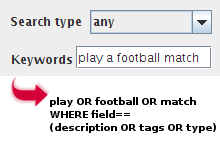
\includegraphics[scale=0.5]{img/query-rich.png}
			\end{figure}
	    
	    \end{column}
	
\end{columns}

\end{frame}


\subsection{Application adaptation \& rules description creation}

\begin{frame}

\frametitle{Application adaptation \& rules description creation}

\begin{columns}

	\begin{column}{6cm}
	
	\begin{itemize}
      	\item Some are performed by the user: choosing rules, changing
      	description, etc.
      	\item Some are performed in a transparent way:
		\begin{itemize}
      		\item It required more analysis.
      		\item I.e.: Modify the ownership of the rules internally for certain
      		nodes.
      		\item Implemented using DOM.
        \end{itemize}
        
	\end{itemize}

		
	
	\end{column}
	
		\begin{column}{6cm}
	    
			\begin{figure}
			 	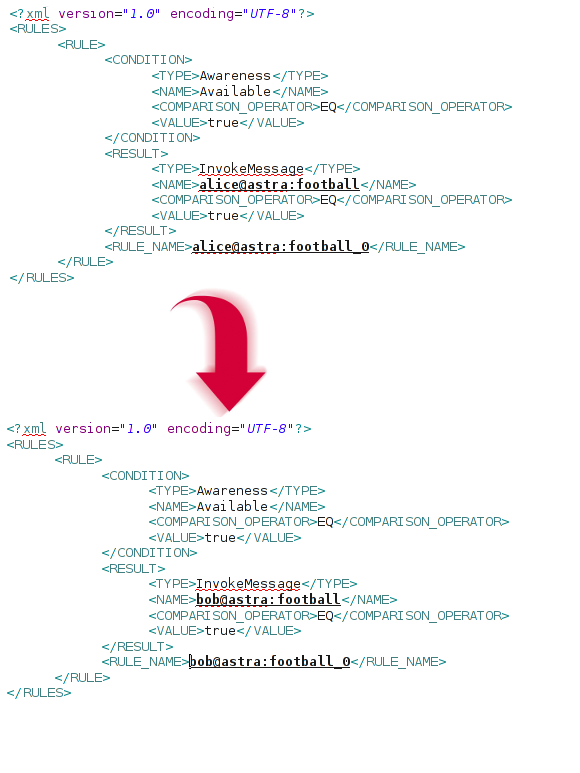
\includegraphics[scale=0.2]{img/rules-transformation.png}
			\end{figure}
	    
	    \end{column}
	
\end{columns}

\end{frame}


\begin{frame}

	\begin{itemize}
	  	\item A similar approach was taken to create a description of the rule
	  	based on the XML file that represents it.
	  	\item I.e.: creating a human readable description for a rule while 
	  	analyzing recursively the tree.
	 \end{itemize}

	\begin{figure}
	 	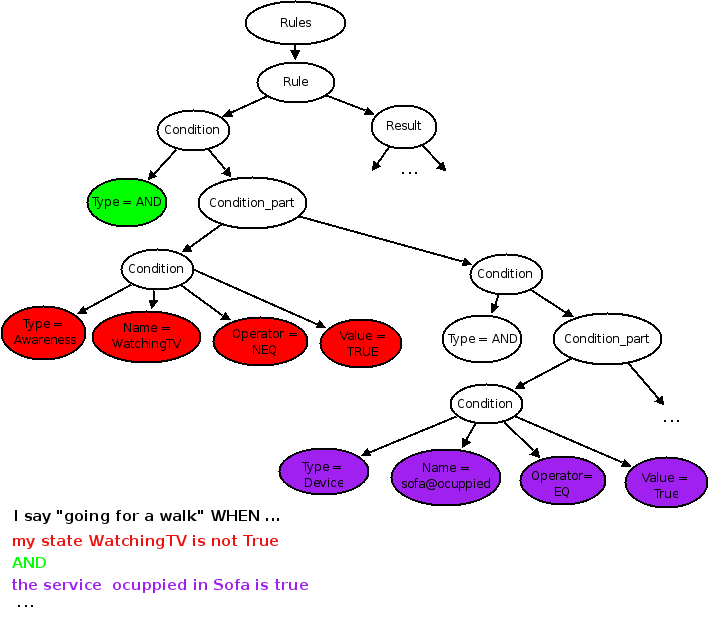
\includegraphics[scale=0.23]{img/rule-tree.png}
	\end{figure}


\end{frame}